\iffalse
\documentclass{article}
% Language setting
% Replace `english' with e.g. `spanish' to change the document language
\usepackage[english]{babel}
% Set page size and margins
% Replace `letterpaper' with `a4paper' for UK/EU standard size
\usepackage[letterpaper,top=2cm,bottom=2cm,left=3cm,right=3cm,marginparwidth=1.75cm]{geometry}
% Useful packages
\usepackage{multicol}
\usepackage{amsmath}
\usepackage{amssymb}
\usepackage{graphicx}
\usepackage[framemethod=tikz]{mdframed}
\usepackage{array}
\usepackage{blindtext}
%\usepackage[paperwidth=10cm]{geometry}
\usepackage{tkz-euclide}
%\usepackage{tikz}
\usetikzlibrary{
  circuits.logic,
  circuits.logic.US,
  positioning
}

\usepackage[colorlinks=true, allcolors=blue]{hyperref}
\newcommand{\myvec}[1]{\ensuremath{\myvec{#1}}}
\providecommand{\norm}[1]{\left\lVert#1\right\rVert}
\let\vec\mathbf
\title{Conic Assignment}
\author{Anusha Jella}
\begin{document}
\maketitle
\newtheorem{theorem}{Theorem}[section]
\begin{multicols}{2}

\paragraph{\begin{flushleft}\textbf{Problem: }
	\fi
Find the equation of all lines having slope  -1 that are tangents to the curve
\begin{align}
y = \frac{1}{x-1}, x \neq 1
\end{align}
	\begin{figure}[!ht]
		\centering
 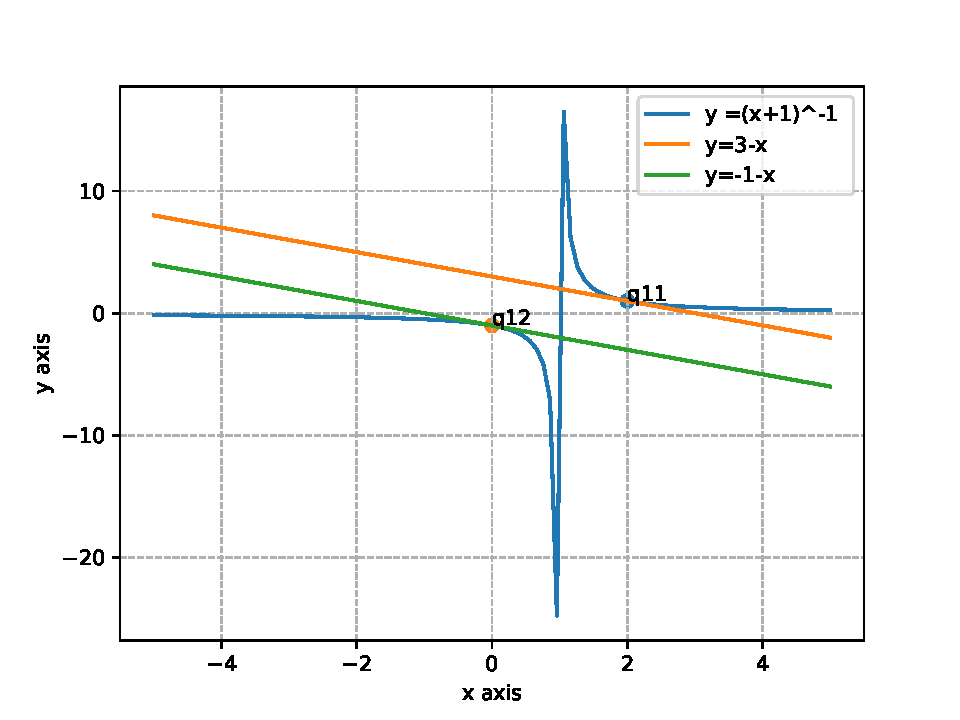
\includegraphics[width=\columnwidth]{chapters/12/6/3/10/figs/conic1.pdf}
		\caption{}
		\label{fig:12/6/3/10}
  	\end{figure}
	\\
	\solution 
\iffalse
\end{flushleft}}
%\begin{figure}[h]
\centering
\includegraphics[scale=0.5]{conic_fig1.pdf} 
%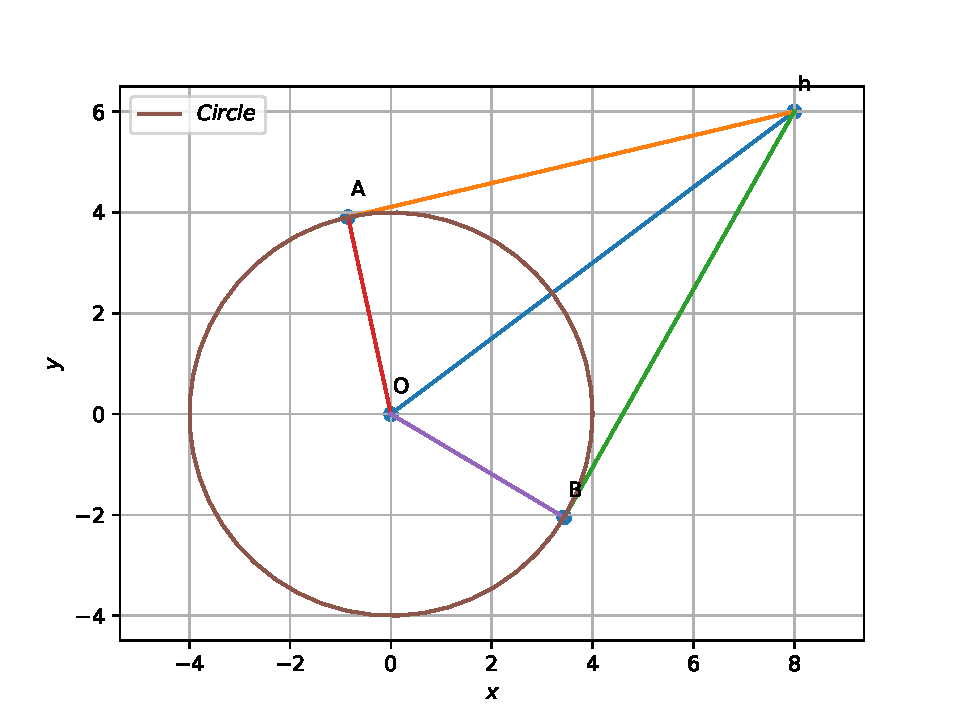
\includegraphics[width=\columnwidth]{circle1.pdf} 
\centering{Fig 1. Curve}
\label{fig:circle_1}
%\end{figure}

 \section*{Construction}
 \begin{flushleft}
 \textsc{solution:} The following python code is used for constructing conic with tangents.
 \end{flushleft}
 \begin{mdframed}
   \url{https://github.com/AnushaJella/assignment_conic/blob/main/conic1.py}\\
\end{mdframed}
See Fig 1 for the input parameters in Table 1.\\
\vspace{0.5cm}
{\setlength\extrarowheight{2pt}
\begin{tabular}{|c|c|c|}
	\hline
	\textbf{Symbol}&\textbf{Value}&\textbf{Description}\\
	\hline
	$\textbf{x}$&[-5,5,100] &to find $\textbf{y}$\\
	\hline
\end{tabular}
}\\
\centering {Table 1}\\
\section*{Solution}
\begin{flushleft}
The equation of  a conic with directrix $\vec{n}^{\top}\vec{x} = c$, eccentricity $e$ and focus $\vec{F}$ is given by 
\end{flushleft}
\begin{align}
    \vec{x}^{\top}\vec{V}\vec{x}+2\vec{u}^{\top}\vec{x}+f=0
    \end{align}
\hspace{-6.5cm}where     
\begin{align}
  \label{eq:conic_quad_form_v}
\vec{V} &=\norm{\vec{n}}^2\vec{I}-e^2\vec{n}\vec{n}^{\top}, 
\\
\label{eq:conic_quad_form_u}
\vec{u} &= ce^2\vec{n}-\norm{\vec{n}}^2\vec{F}, 
\\
  f &= \norm{\vec{n}}^2\norm{\vec{F}}^2-c^2e^2
\end{align}
\hspace{-6.5cm}Given, 
\fi
From the given information, 
\begin{align}
	\vec{V}
	=\myvec{
		0 & \frac{1}{2}\\\frac{1}{2}& 0\\
	},
\vec{u} = \myvec{
0 \\-\frac{1}{2}\\
},  f = -1, m=-1
	\label{eq:matrix-10-13-param}
\end{align}
From the above, the  normal vector is
\begin{align}
\vec{n}=\myvec{
-m \\ 1
	} = \myvec{1 \\ 1}
	\label{eq:matrix-10-13-param-n}
\end{align}
From 
\eqref{eq:conic_tangent_qk},
	the point(s) of contact are given by
\begin{align}
	\vec{q}&=\vec{V}^{-1}(k_i\vec{n}-\vec{u}) 
	\text{ where},\\
	k_i&=\pm \sqrt{\frac{f_0}{\vec{n}^{\top}\vec{V}^{-1}\vec{n}}}\\
	f_0&=f+\vec{u}^{\top}\vec{V}^{-1}\vec{u}
\end{align}
Substituting from 
	\eqref{eq:matrix-10-13-param-n}
	and
	\eqref{eq:matrix-10-13-param}
	in the above,
\begin{align}
\vec{q}=\myvec{0 \\-1}, \myvec{2 \\ 1}.
\end{align}
From 
  \eqref{eq:conic_tangent_final},
the equations of tangents are given by
\begin{align}
(\vec{V}\vec{q}+\vec{u})^{\top}\vec{x}+\vec{u}^{\top}\vec{q}+f=0
\end{align}
yielding
\begin{align}
	\myvec{1 & 1}\vec{x}+1&=0\\
\myvec{1 & 1}\vec{x}-3&=0\\
\end{align}
See Fig. 
		\ref{fig:12/6/3/10}.
\iffalse

\end{multicols}{2}
\end{document}
\fi
